\documentclass{beamer}
\usetheme{Madrid}

\usepackage{amsmath, amssymb, amsthm}
\usepackage{graphicx}
\usepackage[utf8]{inputenc}
\usepackage{hyperref}

\title{11.16.3.6}
\author{EE24BTECH11004 - Ankit Jainar}
\date{\today}

\begin{document}

\frame{\titlepage}

\begin{frame}
\frametitle{Question}
There are four men and six women on the city council. If one council member is selected for a committee at random, how likely is it that it is a woman?
\end{frame}

\begin{frame}
\frametitle{Theoretical Solution}
The total number of council members is:
\[
|S| = 4 + 6 = 10
\]
The favorable outcomes (selecting a woman) are:
\[
|A| = 6
\]
The probability of selecting a woman is:
\[
P(A) = \frac{|A|}{|S|} = \frac{6}{10} = 0.6
\]
\end{frame}

\begin{frame}
\frametitle{Introduction}
This task involves simulating the random selection of council members using:
\begin{itemize}
    \item A C program to generate random samples.
    \item Compiling the program into a shared object (.so) file.
    \item Using Python to process the results and generate a probability distribution plot.
\end{itemize}
\end{frame}

\begin{frame}
\frametitle{C Code Description}
The C program performs the following:
\begin{itemize}
    \item Generates random samples for the selection process.
    \item Uses the \texttt{rand()} function to simulate the random selection.
    \item Tracks the number of outcomes categorized as either "man" or "woman."
\end{itemize}
\end{frame}

\begin{frame}
\frametitle{Python Code Description}
The Python code performs the following:
\begin{enumerate}
    \item Loads the shared object file generated from the C program using the \texttt{ctypes} library.
    \item Simulates a specified number of random selections (e.g., 1,000,000 trials).
    \item Calculates the probability of selecting a woman using the formula:
    \[
    P(\text{woman}) = \frac{\text{frequency of selecting a woman}}{\text{total trials}}
    \]
    \item Plots the probability distribution using \texttt{matplotlib}.
\end{enumerate}
\end{frame}

\begin{frame}
\frametitle{Graphical Output}
The Python code generates a bar chart where:
\begin{itemize}
    \item The x-axis represents the outcomes: Man and Woman.
    \item The y-axis represents the probabilities, ranging from 0 to 1.
    \item The bar height for Woman corresponds to the probability \(P(A) = 0.6\).
\end{itemize}
\end{frame}

\begin{frame}
\frametitle{Probability Mass Function (PMF)}
The PMF represents the probability of each individual outcome in the sample space \(S\).  
For the city council:
\[
S = \{\text{Man, Woman}\},
\]
the PMF is given as:
\[
P(X = x) = 
\begin{cases} 
\frac{6}{10}, & x = \text{Woman}, \\ 
\frac{4}{10}, & x = \text{Man}, \\ 
0, & x \notin S.
\end{cases}
\]
\end{frame}

\begin{frame}
\frametitle{Cumulative Distribution Function (CDF)}
The CDF represents the cumulative probability of outcomes up to a given value \(x\), defined as:
\[
F(x) = P(X \leq x) = \sum_{k \in S, k \leq x} P(X = k).
\]
For the city council:
\[
F(x) = 
\begin{cases} 
0, & x < \text{Man}, \\ 
\frac{4}{10}, & x = \text{Man}, \\ 
1, & x \geq \text{Woman}.
\end{cases}
\]
\end{frame}

\begin{frame}
\frametitle{Simulation Process}
Steps to simulate the selection of a council member:
\begin{enumerate}
    \item The council consists of members in the set:
    \[
    S = \{\text{Man, Woman}\}.
    \]
    \item Generate a random integer \(X\) such that:
    \[
    X \in \{1, 2, \dots, 10\}.
    \]
    \item If \(X \leq 6\), it corresponds to a woman; otherwise, it corresponds to a man.
    \item Track the number of occurrences of each outcome over \(N\) trials.
\end{enumerate}
\end{frame}
\begin{frame}
\begin{figure}[h!]
   \centering
   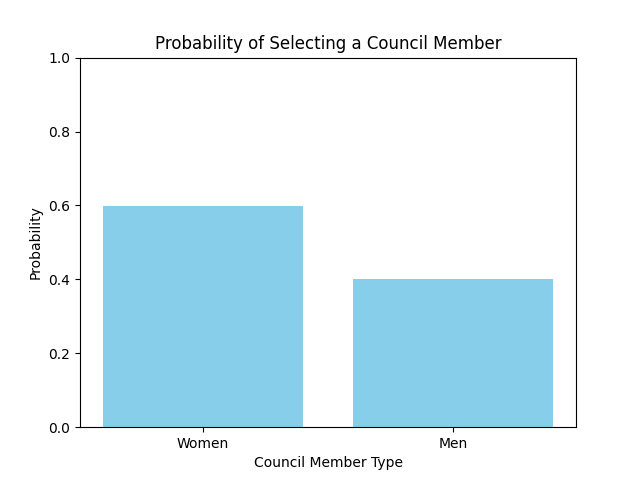
\includegraphics[width=\columnwidth]{figs/fig1.png}
   \end{figure}
\end{frame}  
\begin{frame}
\begin{figure}[h!]
   \centering
   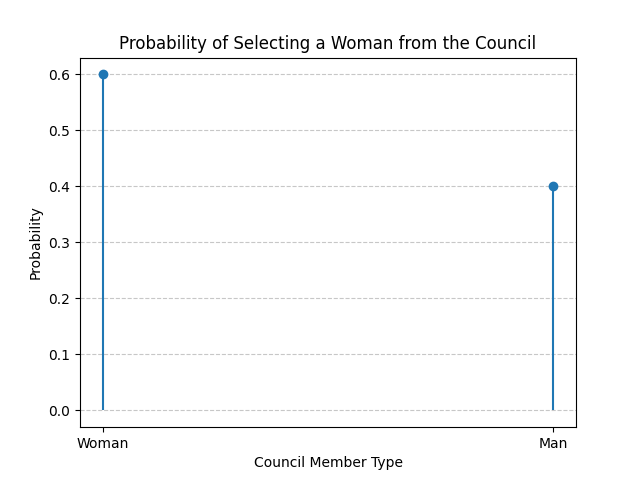
\includegraphics[width=\columnwidth]{figs/fig2.png}
   \end{figure}
\end{frame}   
\begin{frame}
\begin{figure}[h!]
   \centering
   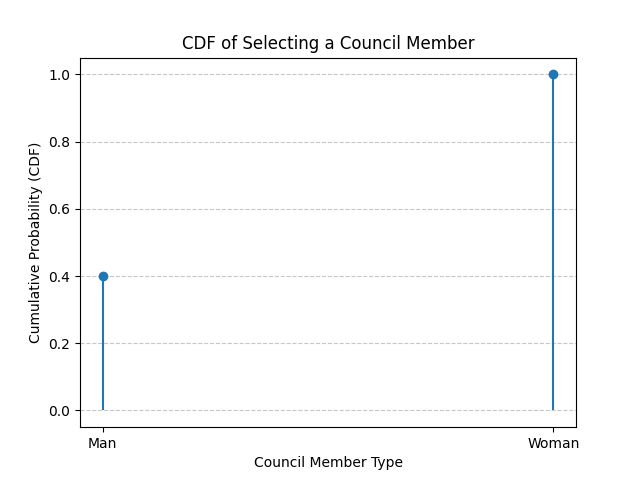
\includegraphics[width=\columnwidth]{figs/fig3.png}
   \end{figure}
\end{frame}
\begin{frame}
\frametitle{Conclusion}
This task demonstrates the integration of C and Python for simulating and visualizing a probabilistic experiment.  
The probability of selecting a woman from the council is calculated as:
\[
P(\text{Woman}) = 0.6,
\]
matching the theoretical value.
\end{frame}

\end{document}

